%%%%%%%%%%%%%%%%%%%%%%%%%%%%%%%%%%%%%%%%%%
%% TEX main file for the CLAS12 Nim Papers
%%       Do not edit this file
%%%%%%%%%%%%%%%%%%%%%%%%%%%%%%%%%%%%%%%%%%
\documentclass[3p,times,twocolumn]{elsarticle}
\usepackage{lineno, hyperref, multicol, multirow, color, xspace, pdfwidgets, enumerate, amssymb, adjustbox}

\modulolinenumbers[5]
\linenumbers

\journal{Nuclear Instruments and Methods A}

\begin{document}

\begin{frontmatter}
\title{CLAS12 High Threshold Cherenkov Counter}

\author[1]{Y.G.Sharabian}
\author[1]{V.D.Burkert}
\author[1]{S.Christo}
\author[1]{C.Cuevas}
\author[1]{H.Dong}
\author[13]{S.Danagoulian}
\author[2]{A.Ellis}
\author[1]{L.Elouadrhiri}
\author[1]{B.Eng}
\author[3]{K.Hafidi}
\author[4]{I.Illari}
\author[1]{G.Jacobs}
\author[5]{K.Joo}
\author[1]{D.Kashy}
\author[6]{A.V.Kubarovsky}
\author[1]{V.P.Kubarovsky}
\author[7]{S.Maiylian}
\author[1]{N.Markov}
\author[1]{M.Mcmullen}
\author[1]{B.Miller}
\author[8]{r.Niyazov}
\author[7]{R.Paremuzyan}
\author[9]{W.Phelps}
\author[1]{V.Popov}
\author[10]{A.Puckett}
\author[1]{B.Raydo}
\author[11]{D.Riser}
\author[12]{P.Stoler}
\author[13]{A.Vlasov}
\author[7]{A.Voskanyan}

\address[1]{Placeholder location}
\address[2]{Placeholder location}
\address[3]{Placeholder location}
\address[4]{Placeholder location}
\address[5]{Placeholder location}
\begin{abstract}

For the 12 GeV upgrade of Jefferson Laboratory, a Silicon Vertex Tracker (SVT) has been designed for the CLAS12 spectrometer using single-sided microstrip sensors fabricated by Hamamatsu. The sensors have a graded angle design to minimize dead areas and a readout pitch of 156 $\mu$m, with intermediate strips. Each double-sided SVT module hosts three daisy-chained sensors on each side with a full strip length of 33~cm. There are 512 channels per module, read out by four Fermilab Silicon Strip Readout (FSSR2) chips, featuring data-driven architecture, mounted on a rigid-flex hybrid board. The modules are assembled on the barrel using a unique cantilevered geometry to minimize the amount of material in the tracking volume. This paper is focused on the design, qualification of the performance, and experience in operating and commissioning the tracker during the first year of the data taking.

\end{abstract}

\end{frontmatter}

\date{\today}

\section{Overview}

simulations overview description, how geometry and digitization.

Then we go to each detector

- geometry
- calibration constants
- digitization.





\section{Requirements}

hallb requirements description


\section{Design}

The CLAS12 Trigger System was designed as a 3-stage pipeline-style system with total latency up to 8~$mu$s. Input information for the Trigger System comes from two sources:  Flash Analog to Digital Converters (FADCs) used in the photomultiplier tube (PMT)-based detectors, and Drift Chamber Readout Boards (DCRBs) used in Drift Chambers. The FADCs and DCRBs work as the pre-trigger level, reporting information to the Trigger System in the appropriate form. Stage 1 receives information from the FADCs and DCRBs and performs data processing according to the type of detector. Stage 2 performs a timing and geometry coincidence between different subsets of detectors in six groups, corresponding to the six-sector CLAS12 detector structure, as well as requires coincidence with information from central detectors. Stage 3 forms the final trigger decision. The CLAS12 Trigger diagram is shown in Fig.~\ref{fig:TriggerDiagram}.

\begin{figure}[hbt]
	\centering
	\includegraphics[width=1.0\columnwidth,keepaspectratio]{img/CLAS12_TRIGGER_1.pdf}
	\caption{The CLAS12 Trigger System diagram.}
	\label{fig:TriggerDiagram}
\end{figure}


\subsection{FADCs as Pre-trigger}

All PMT-based detectors in CLAS12 participating in the Trigger System use JLab VXS 250~MHz flash ADCs as the starting point of the trigger logic (FADC, \cite{daq-ref}). Each channel of the FADC boards is pre-programmed with gain, pedestal, and amplitude threshold above pedestal. Every pulse above amplitude threshold is integrated and sent to the corresponding section of the Stage 1 trigger logic. The 16-channel FADC boards report 13-bit pulse integrals and 3-bit pulse time every 32~ns, which allows the following trigger logic to restore 4~ns pulse resolution while the double pulse resolution remains 32~ns. Based on the FADC reporting schedule, the following trigger logic stages can work on a 250~MHz clock, although in that case we found it problematic to meet the Field Programmable Gate Array (FPGA) timing. Because of that, our Stage 1 algorithms run on 125~MHz or slower clocks as described below. Tteh trigger information is provided to the following stages using VXS backplane serial lines.


\subsection{DCRBs as Pre-trigger}

The Drift Chamber-based trigger uses JLab 125~MHz discriminator/TDC boards (DCRB, \cite{daq-ref}) to feed the Trigger System. These 96-channel units report hits above the pre-programmed thresholds every 16 ns. As for the FADC boards, the DCRBs are implemented in VXS format and provide trigger information using VXS backplane serial lines.


\subsection{Stage 1 Trigger} 

The Stage 1 trigger uses specially designed VXS Trigger Processor boards (VTP, see Section \ref*{sec:vtp_board}). The VTP boards are installed in switch slots in every VXS crate participating in the Trigger System. The VTPs collect trigger data from the pre-trigger boards (FADCs and DCRBs) over VXS serial lines.

The most complex processing is performed for the electromagnetic calorimeters (cluster finding) and the Drift Chambers (segment and road finding). In the following sections we describe the design of the various trigger components.


\subsubsection{Electromagnetic Calorimeters}
\label{sec:ECAL}

The CLAS12 electromagnetic calorimeter (ECAL, \cite{ec-ref}) includes two separate subsystems, the EC and PCAL. Each consists of multiple layers of scintillating strips and lead sheets with photomultiplier readout on one side of the scintillators (the PCAL is shown in Fig.~\ref{fig:PCAL}, the EC is similar). The primary purpose of these detectors is electron identification by defining the energy and coordinate of their electromagnetic showers, referred to as clusters. The cluster finding algorithm was well established during off-line data processing development, and was adopted for the trigger implementation with some simplifications.

The algorithm first searches for one-dimensional clusters in each of the three calorimeter views (u,v,w), sorting them by energy and keeping only those above threshold, with a maximum number of four clusters in each view. Next the algorithm searches for two-dimensional clusters looking for overlap between the three views. For all two-dimension clusters found, it performs attenuation corrections based on pre-loaded tables of the attenuantion lengths of the scintillation strips using the distance from the cluster to the PMT, to deternime the correct cluster energy. Finally, the algorithm sorts the two-dimension clusters by energy and reports those above threshold, with a maximum number limited to four. For every cluster, the energy and coordinates are reported to the Stage 2 trigger every 8~ns. There is a persistency parameter that allows the same clusters to be reported for several consecutive 8~ns intervals to check for a timing coincidence with the other trigger components, as well as a timing delay parameter for the same purpose. One event with a single cluster is shown in the PCAL (preshower calorimeter) in Fig.~\ref{fig:PCAL}. The corrected energies are shown for the individual strips.

It should be mentioned that such an algorithm is designed to find clusters with a maximum energy to target electron identification. For some CLAS12 experiments, it is necessary to identify minimum-ionizing particles (MIPs) using the same trigger component. For that purpose, clusters with energy below a certain defined threshold can be selected. Such a method works for events where the number of clusters does not exceed four, otherwise there is a risk of losing low-energy clusters corresponding to MIPs. Intensive trigger efficiency studies were conducted for such cases, and the MIP trigger efficiency was measured and found acceptable.

\begin{figure}[htp]
	\begin{center}
		\centering
		\includegraphics[width=7cm]{img/pcal1.png}
		%\includegraphics{PCA.pdf}
		\caption{Trigger System representation of a cluster reconstruction using the three views of the PCAL in one sector of CLAS12.}
		\label{fig:PCAL}
	\end{center}
\end{figure} 


\subsubsection{High Threshold Cherenkov Counter}
\label{sec:HTCC}

The CLAS12 High Threshold Cherenkov Counter (HTCC, \cite{htcc-ref}) serves as one of the primary components of the electron trigger logic. It was specially designed to discriminate electrons from other charged particles. The HTCC consists of 48 mirror sections readout by PMTs connected to FADCs (see Fig.~\ref{fig:multihitHTCC}). For trigger purposes, a 2x2 section sliding window is used to identify clusters. The cluster may include from one to four PMT signals collecting the Cherenkov light from the adjacent mirrors as shown in  Fig.~\ref{fig:multihitHTCC}. The configuration parameters include the single channel energy threshold, cluster multiplicity threshold, and cluster energy threshold. The results are reported to the Stage 2 trigger as 48-bit masks every 4 ns. The FADC ``gain'' configuration parameter allows for PMT energy calibrations, making it possible to set energy thresholds in terms of the number of photoelectrons.


\begin{figure}[htp]
	\begin{center}
		\centering
		\includegraphics[width=8cm]{img/multiHits.pdf}
		\caption{Hits registered by the HTCC (red circles) and the reconstructed cluster position (yellow). The hit position and cluster position coincide for one hit clusters (top left plot), which has the lowest position resolution.}
		\label{fig:multihitHTCC}
	\end{center}
\end{figure} 


\subsubsection{Drift Chamber}
\label{sec:DC}

The CLAS12 Drift Chambers (DC, \cite{dc-ref}) contain six superlayers in each of the six CLAS12 sectors. Each superlayer contains six layers, and 112 wires in each layer. There is no signal amplitude information available, only hit information can be used in the trigger. The Trigger algorithm was designed as a two-step process.

In the first step it searches for segments in each of the six superlayers, reporting a 112-bit mask with the bits set for the segments found. The search for segments is conducted based on a pre-loaded segment dictionary, generated by the Drift Chamber simulation software based on the wire locations in the superlayers. If several segments are found in the same location, the one with the maximum number of hits is kept. In theory, the number of layers contributing to each segment must be equal to 6, and the number of hit wires in a segment can vary from 6 to 12 depending on the track position and angle. In practice, the number of layers and hits in each segment can be less because of Drift Chamber inefficiencies and hardware problems, so the threshold for the segment finder in the trigger logic was usually set to 4 and sometimes to 3 layers out of 6 to ensure an efficient trigger.

After the segment search is complete and the six 112-bit masks are ready, the second step is performed, in which a pre-loaded road dictionary (corresponding to all possible charged particle trajectories) is used to identify possible track candidates (so-called road finding). The road disctionaries were generated by the GEMC Monte Carlo simulation program (\ref) or taken from the real beam data (\ref). At least five out of six superlayers are required to satisfy the trigger condition. All found roads are reported to the Stage 2 trigger every 16~ns. The information reported in the form of 112-bit words is used for the geometry match in the Stage 2 trigger.


\subsubsection{Forward Time-Of-Flight System}

The CLAS12 Forward Time-Of-Flight System (FTOF, \cite{ftof-ref}) contains two layers of scintillating counters in each sector, but only one layer is used by the trigger logic. This layer contains 62 counters with PMT readout on both ends. When both PMTs report a signal above threshold, the trigger system considers it as a hit. A 62-bit hit mask is reported to the Stage 2 trigger every 4~ns. The trigger logic configuration includes a single channel energy threshold and a counter average energy threshold (geometry mean). The FTOF participates in non-electron triggers such as the muon trigger.


\subsubsection{Central Time-Of-Flight System}

The CLAS12 Central Time-Of-Flight System (CTOF, \cite{ctof-ref}) consists of 48 scintillation counters, surrounding the target as a barrel, with PMT readout from both ends. Its trigger logic is similar to that for FTOF, with a 48-bit mask reported to the Stage 2 trigger every 4~ns.


\subsubsection{Central Neutron Detector}

The CLAS12 Central Neutron Detector (CND, \cite{cnd-ref}) consists of three layers of scintillation counters, installed radially outward from CTOF, with 24 counters per layer and 72 counters total. Its trigger logic is similar to that for FTOF and CTOF, with a 24-bit mask reported to the Stage 2 trigger every 4~ns (usually the inner layer only).


\subsubsection{Forward Tagger Calorimeter and Hodoscope}

The CLAS12 Forward Tagger Calorimeter and Hodoscope (FT, \cite{ft-ref}) trigger is designed to trigger on electrons at small forward angles (theta from 2deg to 5deg). The calorimeter is a stack of 332 lead tungstate crystals connected to avalanche photodiodes (APDs) that are readout by FADCs. The hodoscope consists of two scintillating fiber layers, each having 116 pixels (of two sizes) that matches the geometry of the calorimeter. The calorimeter trigger finds clusters by looking for a seed hit at each crystal location. If the deposited energy in a crystal is greater than the seed threshold and is a local maximum in space (using a 3x3 crystal view) and time, then it is considered a seed hit. For each seed hit, a cluster is formed by summing all of the energies centered on the seed hit in a 3x3 crystal view for all hit times coincident with the seed hit (up to $\pm$16~ns). The seed hit time, which due to time walk effects is the earliest hit in the cluster, is used for the cluster time stamp, providing a 4~ns resolution. The geometrically matched hodoscope pixels for both layers are checked for time coincident hits with the calorimeter seed hit and the cluster is tagged as having none, layer 1, layer 2, or both layers of the hodoscope present. Found clusters are serialized and streamed to the Stage 2 trigger where several programmable trigger cuts can discriminate clusters based on energy, charge, and multiplicity.


\subsection{Stage 2 Trigger}

The Stage 2 trigger collects data from Stage 1 using fiber optics. It is based on the number of SubSystem Processor boards (SSP, see Section \ref*{sec:ssp_board}) all installed in one VXS crate. After receiving the Stage 1 trigger streams, the SSPs form subsystem coincidences for the six identical sets of forward detectors (called sectors) and the central detectors (all separately). Each subsystem trigger stream goes through a programmable delay that provides 4~ns resolution when deskewing to optimize the time coincidence. Next follows a programmable coincidence window for each subsystem trigger stream, also with a 4~ns step resolution, to ensure that the different subdetector signals will remain stable long enough to form a time coincidence regardless of jitter due to particle time-of-flight, detector response, and trigger jitter. Stage 2 Trigger specifications are shown in Table~\ref{tab:stage_2_specs}.

\begin{table}
\begin{center}
	\begin{tabular}{| l | l |}
		\hline \hline
		Name				& Specification	\\
		\hline
		Latency (Stage 1+2)		& 5~$\mu$s	\\
		Jitter				& 4~ns		\\
		Stage 2 trigger bits		& 8		\\
		Deskew range			& 4~$\mu$s	\\
		Deskew step size		& 4~ns	\\
		Coincidence window range	& 2~$\mu$s	\\
		Deskew step size		& 4~ns	\\
		\hline \hline
	\end{tabular}
\end{center}
\caption{Stage 2 Trigger Specifications}
\label{tab:stage_2_specs}
\end{table}

The forward detectors in the trigger consist of FTOF, EC, PCAL, HTCC, and DC. A single SSP collects all forward detector trigger streams from a single sector of CLAS12. After the delay and concidence widths are applied to each input stream, the input streams are copied to 8 programmable sector trigger bits. Each sector trigger bit contains a variety of trigger primitives and customizeable thresolds/cuts that can be tailored for a particular trigger type. The sector trigger bits are computed and sent to the final Stage 3 trigger. Forward Detector Trigger primitives are shown in Table~\ref{tab:fd_trig_primitives}.

\begin{table}
\begin{center}
	\begin{tabular}{| l | l |}
		\hline \hline
		Primitive Name			& Trigger Bit Parameters	\\
		\hline
		PCU     			& Mask				\\
		FTOF    			& Mask				\\
		PCAL				& Cluster Emin, Emax		\\
		ECAL				& Cluster Emin, Emax		\\
		PCAL+ECAL			& Cluster Emin			\\
		HTCC				& Mask				\\
		{\bf Geometry Matched}		&				\\
		PCUxFTOF			& Bar match tolerance		\\
		PCALxDC				& Cluster Emin			\\
		\hline \hline
	\end{tabular}
\end{center}
\caption{Forward Detector Trigger Primitives}
\label{tab:fd_trig_primitives}
\end{table}

The central detectors participating in the trigger consist of CTOF, CND, and FT. A single SSP collects all central detector trigger streams. After the delay and concidence widths are applied to each input stream, the input streams are copied to 8 programmable central trigger bits. Each central trigger bit contains a variety of trigger primitives and customizable thresolds/cuts that can be tailored for a particular trigger type. The central trigger bits are computed and sent to the final Stage 3 trigger where all sector and central trigger bits arrive to compute the global trigger bits. Central Detector Trigger primitives are shown in Table~\ref{tab:cd_trig_primitives}.

\begin{table}
\begin{center}
	\begin{tabular}{| l | l |}
		\hline \hline
		Primitive Name			& Trigger Bit Parameters	\\
		\hline
		CND     			& Mask				\\
		CTOF    			& Mask				\\
		FT				& Cluster Emin, Emax, 		\\
						& Cluster Size, Hodoscope	\\
		{\bf Geometry Matched}		&				\\
		CNDxCTOF			& Bar match tolerance		\\
		\hline \hline
	\end{tabular}
\end{center}
\caption{Central Detector Trigger Primitives}
\label{tab:cd_trig_primitives}
\end{table}


\subsection{Stage 3 Trigger}

The Stage 3 trigger is the final stage and collects all sector and central trigger bit streams in a single module where they can be combined in a variety of ways to generate the global trigger bits used for reading out the Data Acquisition System (DAQ). It is implemented on a single VTP board installed in the switch slot on the same VXS crate where all Stage 2 trigger SSPs reside. There are 32 independent trigger bits that can form a trigger based on any combination of sector and/or central trigger bits. Each trigger bit contains two sector trigger bit conditions (required to both be true) and a signle central trigger bit condition. Additionally, each trigger bit contains a 16~bit prescaler, final pulse width, and scaler. Stage 3 Trigger specifications are shown in Table~\ref{tab:stage_3_specs}.

\begin{table}
\begin{center}
	\begin{tabular}{| l | l |}
		\hline \hline
		Name				& Specification	\\
		\hline
		Latency (Stage 1+2+3)		& 7~$\mu$s	\\
		Jitter				& 4~ns		\\
		Stage 3 trigger bits		& 32		\\
		Prescaler			& 0-65535	\\
		Trigger bit width		& 4~ns - 1~$\mu$s	\\
		Pulse rate			& 0.05~Hz - 125~MHz	\\
		\hline \hline
	\end{tabular}
\end{center}
\caption{Stage 3 Trigger Specifications}
\label{tab:stage_3_specs}
\end{table}


\subsection{Trigger Information in Data Stream}
\label{sec:trigger_in_datastream}

An important part of the Trigger System is the Event Builder, which allows the trigger components to participate in event-by-event readout the same way as is done for the DAQ components. All three stages of the Trigger System are equipped with Event Builders. Every time the CLAS12 DAQ is triggered, Stage 1 will build the data bank(s) with trigger decision details (such as the ECAL cluster coordinate/energy or DC segments/roads information), Stage 2 will build the data bank with sector-level and central detector coincidence results, and Stage 3 will build the data bank that contains the trigger bit decisions for all final 32 trigger bit decisions. Event Builders read information from the pipeline-style buffers for a given programmable window related to the readout trigger time. All trigger-related data banks are available in the data stream along with the DAQ data banks, providing detailed information about the trigger decision for every accepted event. In particular, this allows the Trigger System to be run in ``tagging mode'', which is a powerful way to test the trigger efficiency (using either a loose or a random trigger).

\section{Hardware Components and Constructions}

template Hardware Components and Constructions description


\section{Software}



\subsection{Development Software}

Several software packages were used to implement and test the trigger logic developed for CLAS12. These were the FPGA synthesis and implementation, FPGA high level synthesizer, and FPGA simulation software packages.

For FPGA synthesis and implemenation Xilinx ISE/Planahead and Vivado were used. Most of the front-end boards were developed years ago and use Virtex 5 and Spartan 6 FPGAs, which are not supported by Xilinx Vivado, so we relied on Xilinx ISE/Planahead for synthesis and implementation. Even though these tools are no longer updated by Xilinx they have proved to be stable, reliable, and deliver consistent results. Newer design use Xilinx 7-series parts (we used Artix, Kintex, and Virtex) so we used the Vivado tools, which had far better support than ISE/Planahead.

Vivado HLS was used to implement a variety of trigger algorithms, event builder logic, and general purpose logic. HLS components were able to be verified with C/C++ test benches on their own without anything more than GNU GCC and associated C/C++ header files from the HLS toolchain. This tool often allowed for faster implementation for FPGA implemenation, but many components still were implemented in HDL were resource and/or timing requirements become critical.

A cycle accurate simulation was setup to model, test, and debug the full trigger system was setup using Aldec Riviera. Using this tool we were able to perform simulations using the full trigger system in a mixed language environment (VHDL, Verilog, C/C++) for all FPGA componenets (Xilinx series 5, 6,and 7 components). VHPI was used to interface external C/C++ programs from the DAQ to the VHDL testbench. Using VHPI, calls to the DAQ EVIO C/C++ libraries were possible from VHDL making it possible to feed detector waveform data into the trigger simulation directly from monte-carlo and beam data files. Simulation intensive components, such as SerDes components, were replaced with fast and simple models once verified to improve the performance. The simulator is single-threaded and requires a license for each running instance, making it cost prohibitive to parallelize. Even so, it was capable processing 1 event every ~30 seconds on a typical desktop PC simulating the forward and central trigger system comprised of 24,192 drift chamber wires and ~3400 FADC250 channels.


\subsection{Operating Systems} Moffit

Stage 1 and stage 3 of the CLAS12 Trigger System controlled through Arch Linux running in Xilinx arm ...

Stage 2 controlled by CentOS Linux running on Intel controller. As results all 3 stages designed to provide convenient access to ...
using c/c++ programs.


Archlinux with armv7

\begin{itemize}
\item Linux Kernel 4.4.0
  \begin{itemize}
  \item Updates with specific support for Xilinx products
  \item Availaable at https://github.com/Xilinx/linux-xlnx.git
  \item Custom device-tree
  \item Provides FPGA programming interface
  \item Allocates Physical Memory for use with DMA and event buffers.
  \item Standard I^2c and SPI API.
  \end{itemize}

\item Archlinux compiled for armv7
  \begin{itemize}
  \item Available at https://archlinuxarm.org/
  \item Filesystem over NFS.
  \item diskless booting using tftp
  \end{itemize}

\end{itemize}



\subsection{Configuration Software}

\subsubsection{Configuration Files} sergey

CLAS12 Trigger system has large amount of parameters controlling its logic. Those parameters are set by writing values to hadrware registers, and controlled by reading those registers back. System is using ascii files, example is shown on (Fig.). Every line contains key word and the number of corresponding parameter values. Directive 'include' allows to use hierarhical set of configuration files. Normally main configuration file is selected during run startup procedure, and run control software resolves all 'include' directives creating one big configuration file. That file is used to program all trigger harwdare registers, and it is also written to the data stream for bookkeeping purposes. Register contents are read back and results recorded into data stream as well, providing full control of trigger system settings. Normally the same configuration files contains DAQ settings as well, makeing it complete source for entire DAQ/Trigger system settings.


\subsubsection{Timing Setting}

\begin{figure}[hbt]
	\centering
	\includegraphics[width=1.0\columnwidth,keepaspectratio]{img/delay_scan_ctof_ft.png}
	\caption{CTOFxFT Delay Scan}
	\label{fig:delay_scan_ctof_ft}
\end{figure}

One of the important components of the trigger setting process is delay curves measurements. For that purpose software procedure was developed. It includes special trigger configuration file and software tools to sweep individual subsystem latencies, record set of beam current normalized scalers, and produce corresponding delay plots Fig.~\ref{fig:delay_scan_ctof_ft}. Time trigger time setting detector was kept at a constant value, which determined the DAQ readout window timing, while the other subsystems were changed step by step to monitor the delay curve. Delays and coincidence widths were adjusted to account for known jitter sources to ensure no events are lost due poor timing alignment. This procedure was repeated every time trigger logic was changed.


\subsubsection{Gain calibration and Threshold settings}

One of the important settings in trigger system is FADC ones. As it stated above FADC boards serves as initial stage of the most of the Stage 1 trigger components (except Drift Chamber), and correct pedestal and gain calibration is critical for correct trigger system performance. Pedestal and gain measurements were conducted before run startup, and values were loaded using configuration files. As result, all thresholds in configuration files were set using understandable units such as MeV for calorimeters and the number of photoelectrons for cherenkov counter.

\section{Network}

The CLAS12 network is shown in Fig.~\ref{fig:network_diagram}. Its main component is an Arista router that serves as the backbone for the entire system. The set of main DAQ servers is connected directly to the router by 40~Gbit links. Some front-end components with particularly high data rates are connected directly to the router by 10~Gbit links. Most of the front-end conponents, as well as the workstations are connected to the network switches using 1~Gbit links, while those switches are connected to the router by 10~Gbit links. Two 40~Gbit uplinks connect the entire system to the JLab Computer Center.

Most of the 1~Gbit links use copper wiring, while the 10~Gbit and 40~Gbit links use optic fibers, with the exception of short range server links where 40~Gbit wires are used.

The CLAS12 network shows adequate performance and a high level of reliability. With the projected CLAS12 data rates, it can be used ``as is'' for the foreseeable future.

\begin{figure}[hbt]
	\centering
	\includegraphics[width=1.0\columnwidth,keepaspectratio]{img/CLAS12_NET_1.jpg}
	\caption{CLAS12 DAQ Network Diagram}
	\label{fig:network_diagram}
\end{figure}

\section{Slow Controls}

The CLAS12 slow controls system was heavily upgraded for the 12 GeV era at JLab.  It incorporates legacy and modern hardware and standalone controls systems into full EPICS integration, such that everything is accessible from a single interface and on any computer in the CLAS12 system.  Another important aspect is leveraging standard infrastructure tools supported by central JLab computing resources, for a manageable and reliable controls system.

The CLAS12 slow controls system is based on Experimental Physics Industrial Control System (EPICS), currently version 3.14.12.5 \cite{epics-website}, and includes about 90 EPICS input-output controllers (IOCs) interfacing with approximately 50 different types of hardware via various communication protocols and 100K(?) process variables (PVs).

The controls system monitors and controls all aspects of the CLAS12 detector, beamline, and magnet systems, with monitoring on the data-acquisition system.  This includes voltage supplies from a variety of manufacturers, programmable logic controllers, cryogenic and gas systems, multiple scaler hardwares, flasher sytems, all of the VXS crates, trigger system performance, beamline motors, with sequencing for more complex operations like polarimetry and magnet hystereses.  An example of the superconducting torus magnet's nitrogen system and 10 kHz EPICS monitoring is shown in Figure \ref{fig:tordaq}, and one of the scaler displays covering multiple CLAS12 detector systems is shown in \ref{fig:jlabscalers}.

\begin{figure}[htbp]\centering
\includegraphics[angle=270,width=8cm]{img/fd-scalers}
\caption{And example of the JLab FADC250 scalers for CLAS12 PMT-based detector systems.\label{fig:jlabscalers}}
\end{figure}

\begin{figure}[htbp]\centering
\includegraphics[angle=270,width=8cm]{img/tordaq}
\caption{The 10 kHz EPICS-based readout of superconducting magnet's quench detection system.\label{fig:tordaq}}
\end{figure}

Most of the IOCs run on standard rack-mounted servers running Red Hat Enterprise 7 (RHEL7) in the control room.  A few IOCs run in more speciazed systems in the experimental hall, such VxWorks 5.X real-time operating systems on Motorolla VME controllers, primarily for high-rate, synchronous beam monitoring and support of legacy components.  All IOCs and associated processes are managed with procServ for interactive access when necessary and cronjobs for automatic startup and recovery \cite{procserv-website}.

For the graphical user interface we chose the modern Control Systems Studio (CS-Studio) developed at Oak Ridge National Laboratory \cite{css-website}.   CS-Studio is an Eclipse-based suite of tools for developing and monitoring large scale control systems.  It includes various features supporting quick interface development, such as templating and dynamic generation.  We also use CS-Studio's alarm system, which is based on a mysql database for storing alarm configuration and status and message history, and a server monitoring the IOCs, updating the database, and communicating with clients.  The clients include a graphical interface tightly integrated with the rest of the controls system, with visible feedback and heirarchical view of the alarm system, an annuciator service running in the background in the control room, and a notifier service sending emails to on-call experts on particular alarm conditions.

The operators of the controls system run directly on desktop PCs running RHEL7.  Full remote access is also provided, via 2-factor authentication and X-forwarding or VNC as well as VMWare virtual machines supported by JLab.  Read-only access in a web browser is provided via WebOPI, another product affiliated with CS-Studio.

We utilize two internal EPICS channel access gateways, one read-only for the web interface, and the other for minimizing connections to superconducting magnet controls systems.  Wherever appropriate, the standard autosave feature of EPICS is utilized to automatically preserve settings across IOC reboots, and the standard burt save/restore mechanisms.  The controls system also utilizes many custom hardware and software interlocks.

An important component of the slow controls system is archiving data.  For this we utilize the EPICS archiving system called Mya, a product developed by and in support of accelerator operations at Jefferson Lab and shared with the experimental halls.  This provides storage and access to many previous years data of all CLAS12 EPICS PVs \cite{mya}.

Installation and configuration of the associated desktop and server machines, including custom service daemons, cron jobs, IOCs, network disk mounting, and deployment of upgrades and software changes, is managed via puppet and a central server maintained by Jefferson Lab \cite{puppet-website}.  Resulting maintainence is almost hands-free, and recovery from hardware failures or power outages is largely automated.  Monitoring of the servers is performed with Nagios, also provided by Jefferson Lab, which provides email notifications on system errors \cite{nagios-website}.


\section{Performance}

ec performance description


\section{Conclusions}

To address the change of its scope from electron to pion identification for momenta greater than 3.5~GeV,
the original CLAS Cherenkov Counters were refurbished at part of the new CLAS12 Low Threshold Cherenkov
Counter (LTCC) system. The work included improvements of the reflectivities for the mirrors and the Winston
cones, p-terphenyl coating of the PMTs, expansion of the gas volumes, and redesign of the box walls and patch
panels. The LTCC detector sectors after refurbishment are shown in \F{ltccInstalled} installed on the CLAS12
Forward Carriage upstream of the Forward Time-of-Flight system. The average LTCC efficiency for electron
detection in the momentum range from 3.5 to 6.5~GeV is 94\%. The pion efficiency starts around 50\% near
the expected signal threshold, and rises with momentum as expected. A plateau of 88\% is reached at a momentum
of 5~GeV. This is within range of an expectation of efficiency above 90\%. Additional future studies are required
to full quantify the detection efficiency of the CLAS12 LTCC for both positive and negative pions as a function of
momentum.

\begin{figure}
    \centering
    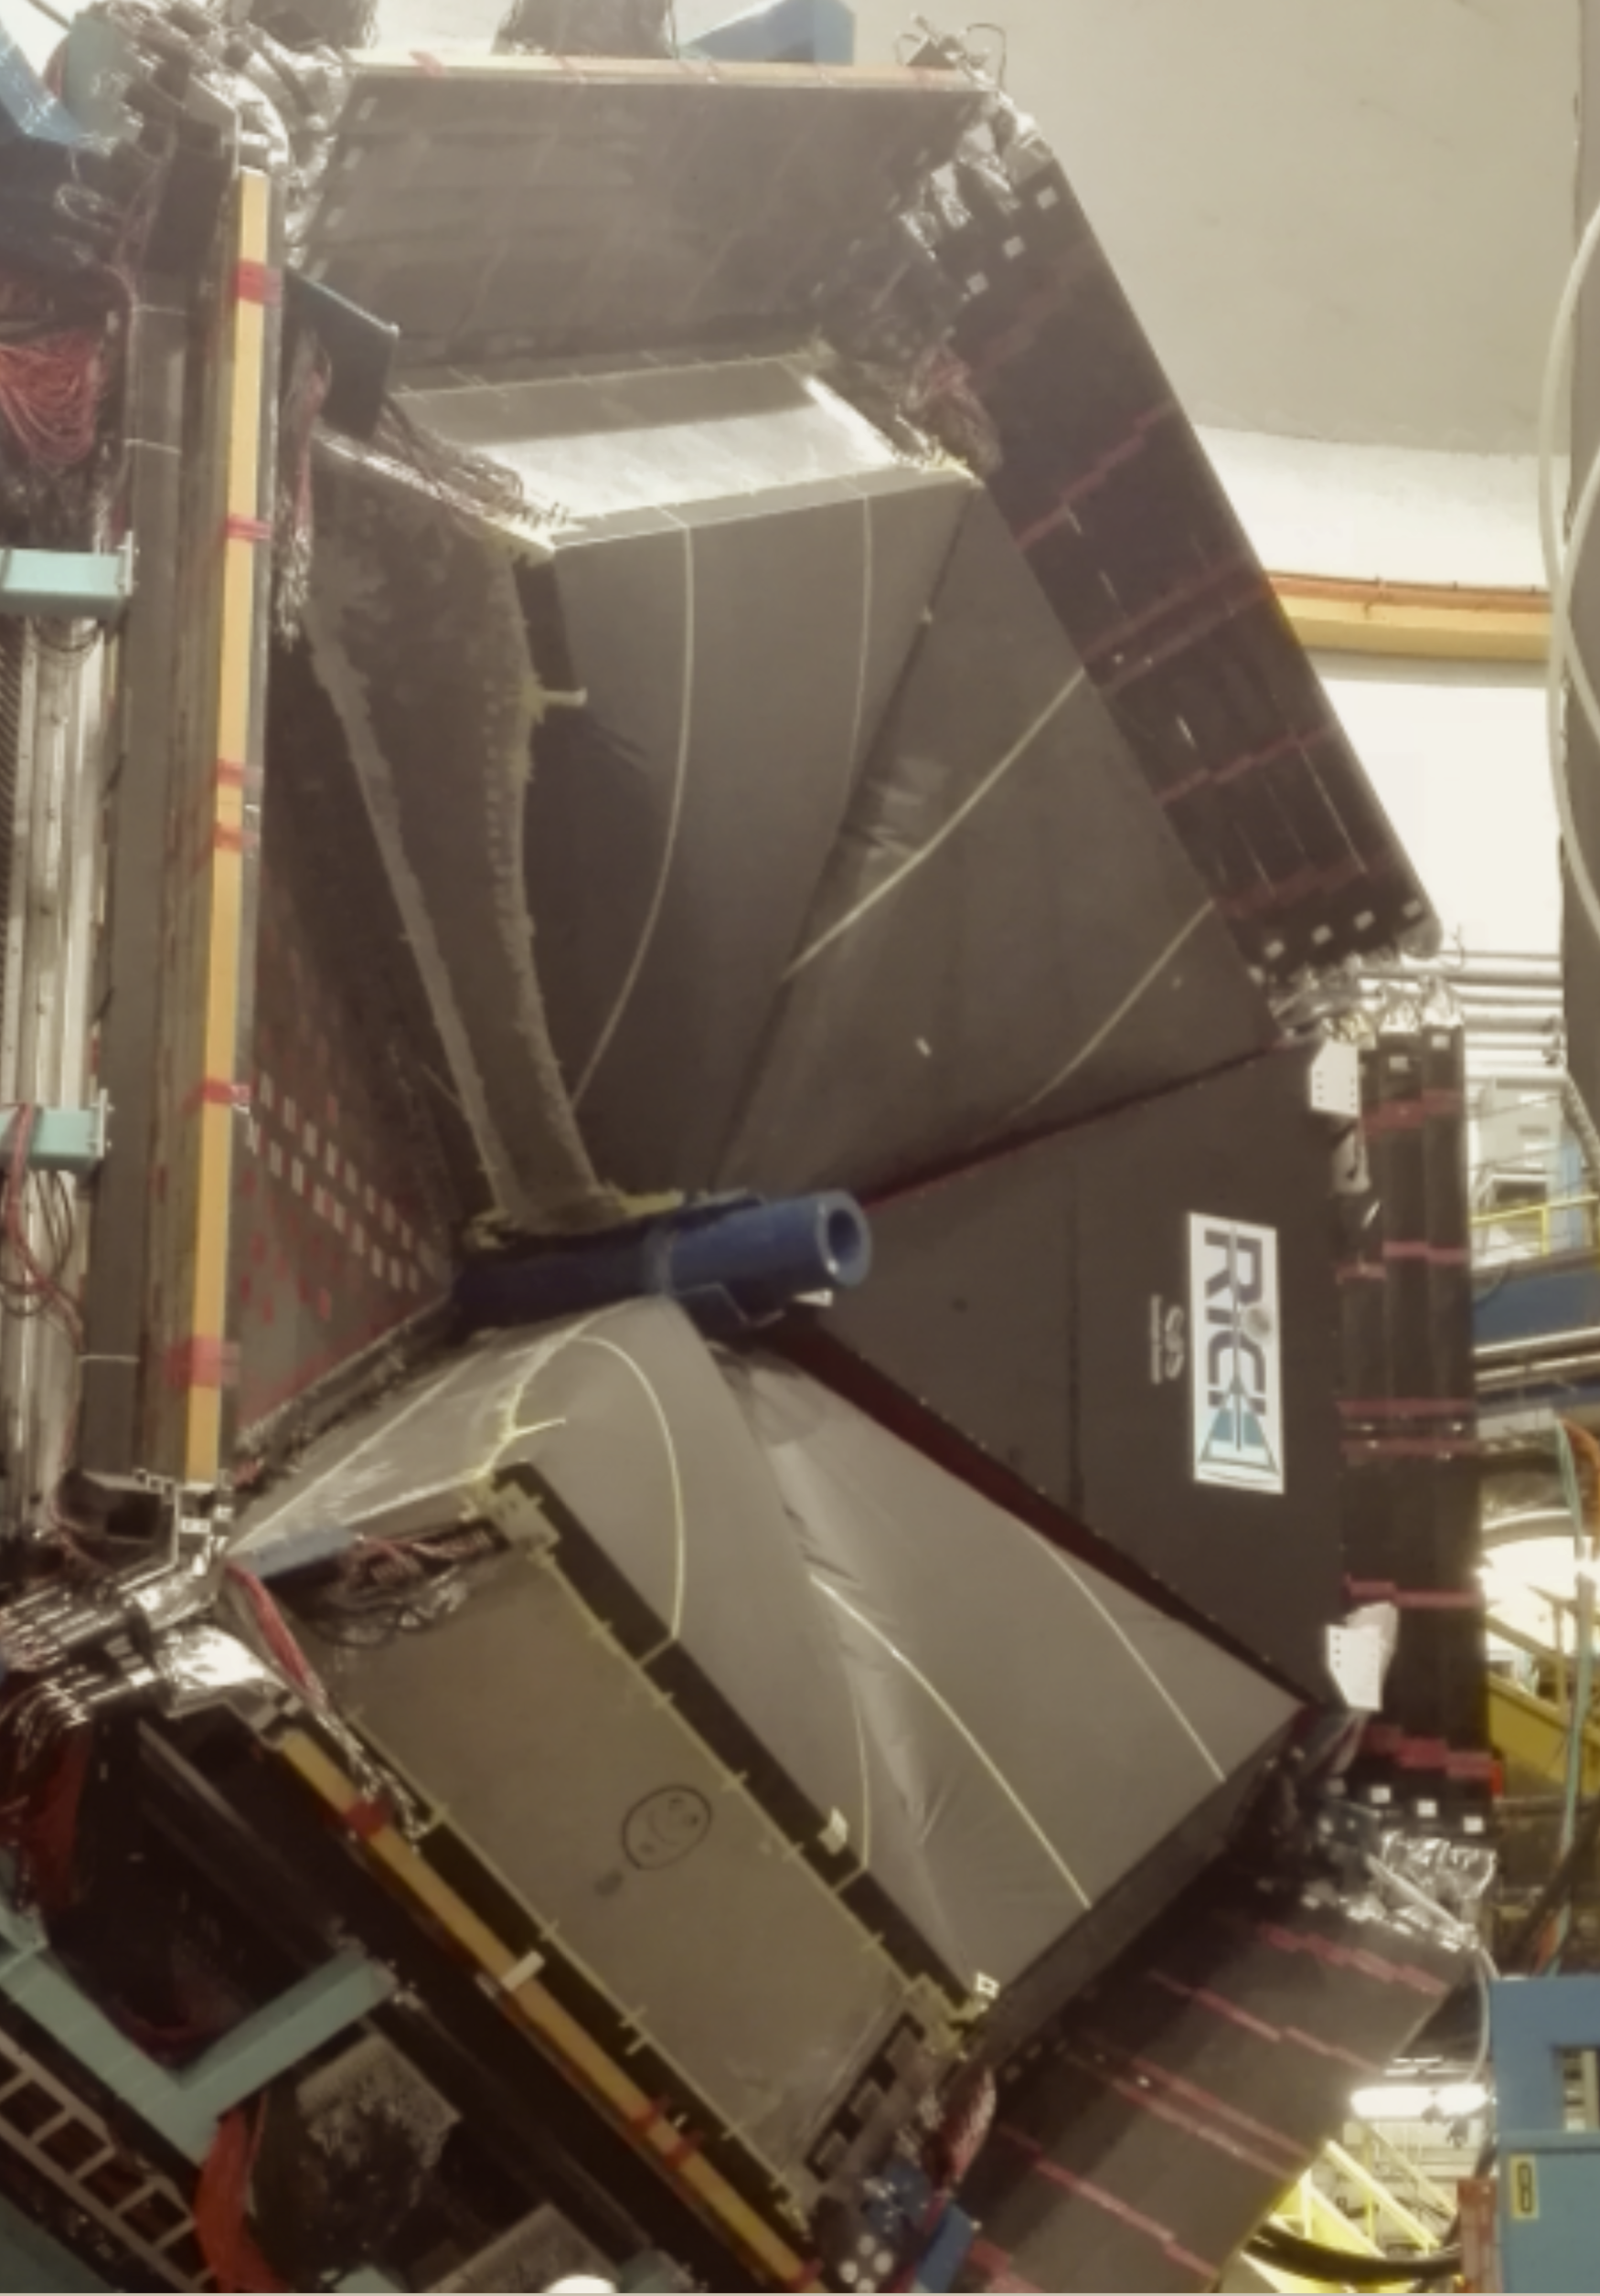
\includegraphics[width=1.0\columnwidth,keepaspectratio]{img/ltccInstalled.png}
    \caption{The LTCC sectors installed after refurbishment on the CLAS12 Forward Carriage. The RICH detector
    is installed in the sector~4 position and the sector~1 position awaits the installation of a second RICH detector.}
    \label{fig:ltccInstalled}
\end{figure}

\section{Acknowledgments}

We thank the Detector Support Group at Jefferson Lab for the work on the cone refurbishment, reflectivity tests,
PMT divider modifications and installation, and for designing the gas control system and associated software. We
thank Temple University for the p-terphenyl deposition. We thank Vladimir Popov for the implementation of the
divider base modification. We thank Youri Sharabian and Steve Christo for their consultations and contributions.
We thank the technical team of Hall~B for their work and dedication on all aspect of the project. Finally, we thank
all the Hall~B staff for their unyielding support. This work was supported in part by
DOE Contract DE-AC05-84ER40150.


\section{References}

%%\bibliography{bibfile}
%%\bibliographystyle{elsarticle-num}

\begin{thebibliography}{99}

	\bibitem{clas-nim}
	B.A. Mecking {\it et al.}, Nucl. Inst. and Meth. {\bf A503}, 513 (2003).
	
	\bibitem{tcs-ref}
	XXX {\it et al.}, {\it ``The YYY Boards''}.
	
	\bibitem{ti-ref}
	XXX {\it et al.}, {\it ``The TI Board''}.

	\bibitem{td-ref}
	XXX {\it et al.}, {\it ``The TD Board''}.

	\bibitem{ts-ref}
	XXX {\it et al.}, {\it ``The TS Board''}.

	\bibitem{sd-ref}
	XXX {\it et al.}, {\it ``The SD Board''}.

	\bibitem{fadc-ref}
	XXX {\it et al.}, {\it ``The FADC Board''}.

	\bibitem{dsc2-ref}
	XXX {\it et al.}, {\it ``The DSC2 Board''}.

	\bibitem{dcrb-ref}
	XXX {\it et al.}, {\it ``The DCRB Board''}.

	\bibitem{vscm-ref}
	XXX {\it et al.}, {\it ``The VSCM Board''}.

	\bibitem{tdc-ref}
	XXX {\it et al.}, {\it ``The TDC Board''}.

	\bibitem{ssp-ref}
	XXX {\it et al.}, {\it ``The SSP Board''}.

	\bibitem{coda-ref}
	XXX {\it et al.}, {\it ``The CODA System'}.

	\bibitem{svt-ref}
	XXX {\it et al.}, {\it ``The CLAS12 SVT Detector'}, see this issue.

	\bibitem{trig-ref}
	B.Raydo {\it et al.}, {\it ``The CLAS12 Trigger System'}, see this issue.

\end{thebibliography}

\end{document}








